% ---------------------------------------------------------------------------
% fig:framework -- Mind World Model overview.
% Both frames sit on top and are carried straight down through the image
% encoder into their visual states; the prediction chain then runs across
% between the two states and meets at the loss.
% ---------------------------------------------------------------------------
\begin{tikzpicture}[x=1cm,y=1cm]

\tikzset{
  ptitle/.style ={font=\normalsize\bfseries, text=inkgray, anchor=north west,
                  inner sep=0pt},
  note/.style   ={font=\scriptsize, text=inkgray!80, inner sep=1.5pt},
  opnode/.style ={circle, draw=inkgray!80, fill=white, line width=0.7pt,
                  inner sep=0pt, minimum size=10pt, font=\scriptsize},
  jdot/.style   ={circle, inner sep=0pt, minimum size=3pt},
  shot/.style   ={inner sep=0pt, draw=inkgray!45, line width=0.6pt},
  onshot/.style ={lbl, anchor=south, inner sep=1.5pt, fill=white,
                  fill opacity=0.80, text opacity=1},
}
% square patch grid, centred on (0,0): #1 = n, #2 = cell, #3 = fill, #4 = stroke
\newcommand{\pgridc}[4]{%
  \pgfmathsetmacro{\gh}{#1*#2/2}
  \foreach \gi in {1,...,#1}{\foreach \gj in {1,...,#1}{
     \fill[#3, draw=#4, line width=0.25pt]
       ({(\gi-1)*#2-\gh},{\gh-(\gj-1)*#2}) rectangle ({\gi*#2-\gh},{\gh-\gj*#2});}}}

% =========================== panel grounds ================================
\path[panel] (-0.14,3.28) rectangle (13.54,8.32);    % (a) world model
\path[panel] (-0.14,0.32) rectangle (13.54,3.16);    % (b) mind model

% ========================= (a) world model ================================
\node[ptitle] at (0.16,8.13) {(a) World model};

% ---- left column: the current frame drops into its visual state ----------
\node[shot] (fanchor) at (1.62,7.00) {
\includegraphics[width=1.24cm]{ego_anchor}};
\node[onshot] at (1.62,6.44) {$\mathbf{I}_t$};
\node[tag, anchor=west] at (2.32,7.00) {current frame};
\node[frozen] (genc) at (1.62,5.86) {\frostlabel{$g$}};
\node[tag, anchor=west, align=left] at (2.08,5.86) {image\\encoder};
\begin{scope}[shift={(1.62,5.02)}] \pgridc{5}{0.11}{vizlight}{vizteal!55} \end{scope}
\node[lbl, anchor=north] at (1.62,4.66) {$\mathbf{S}_t$};
\node[tag, anchor=north] at (1.62,4.26) {visual state};
\draw[vflow] (1.62,6.38) -- (1.62,6.13);
\draw[vflow] (1.62,5.59) -- (1.62,5.32);

% ---- right column: the future frame drops into the target state ---------
\node[shot] (ftarget) at (11.78,7.00) {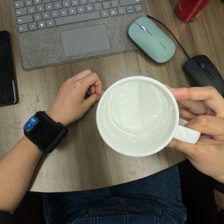
\includegraphics[width=1.24cm]{ego_target}};
\node[onshot] at (11.78,6.44) {$\mathbf{I}_{t+1}$};
\node[tag, anchor=east] at (11.08,7.00) {future frame};
\node[frozen] (gtgt) at (11.78,5.86) {\frostlabel{$g$}};
\begin{scope}[shift={(11.78,5.02)}] \pgridc{5}{0.11}{softgray}{inkgray!40} \end{scope}
\node[lbl, anchor=north] at (11.78,4.66) {$\mathbf{S}_{t+1}$};
\node[tag, anchor=north] at (11.78,4.26) {true next state};
\draw[vflow] (11.78,6.38) -- (11.78,6.13);
\draw[vflow] (11.78,5.59) -- (11.78,5.32);

% ---- the prediction runs between the two states -------------------------
\node[vmod, minimum width=2.25cm, minimum height=0.98cm, align=center]
     (pphi) at (4.62,5.02) {$p_{\phi}$\\[1pt] \scriptsize frame predictor};
\node[opnode] (plus) at (6.35,5.02) {$+$};
\begin{scope}[shift={(7.42,5.02)}] \pgridc{5}{0.11}{vizlight}{vizteal!55} \end{scope}
\node[lbl, anchor=north] at (7.42,4.66) {$\hat{\mathbf{S}}_{t+1}$};
\node[tag, anchor=north] at (7.42,4.26) {predicted state};
\node[lossbox, minimum width=2.30cm, minimum height=0.98cm, align=center]
     (lpred) at (9.55,5.02) {$\mathcal{L}_{\mathrm{pred}}$\\[1pt] \scriptsize prediction loss};

\draw[vflow] (1.92,5.02) -- (3.45,5.02);
\node[lbl, anchor=south, text=inkgray!75] at (2.45,5.12) {$P\!\times\!D_v$};
\draw[vflow] (5.79,5.02) -- (6.20,5.02);
\draw[vflow] (6.51,5.02) -- (7.12,5.02);
\draw[lossflow, draw=losspur!80] (7.73,5.02) -- (8.36,5.02);
\draw[lossflow, draw=losspur!80] (11.48,5.02) -- (10.74,5.02);

% residual skip, routed below the chain so it crosses nothing
\node[jdot, fill=vizteal] at (3.10,5.02) {};
\draw[vflow, draw=vizteal!70] (3.10,5.02) -- (3.10,6.30) -- (6.35,6.30) -- (6.35,5.19);
\node[lbl, text=vizteal!85!black, anchor=south] at (4.75,6.34) {residual $\mathbf{S}_t$};

% ---- the EEG enters only as modulation ----------------------------------
\node[note, anchor=west] at (0.30,3.62)
  {AdaLN modulation\ \ $\gamma(\mathbf{a}_t),\,\beta(\mathbf{a}_t)$};

% ========================= (b) mind model =================================
\node[ptitle] at (0.16,2.98) {(b) Mind model};

\fill[eeglight, draw=eegblue!35, line width=0.6pt, rounded corners=2pt]
      (0.25,0.95) rectangle (2.30,2.10);
\begin{scope}
  \clip (0.25,0.95) rectangle (2.30,2.10);
  \begin{scope}[shift={(0.25,1.96)},xscale=1.42] \eegtrace{2.20}{1.00}{5}{eegblue} \end{scope}
\end{scope}
\begin{scope}
  \clip (2.30,0.95) rectangle (2.82,2.10);
  \begin{scope}[shift={(0.25,1.96)},xscale=1.42] \eegtrace{2.20}{1.00}{5}{eegblue!24} \end{scope}
\end{scope}
\node[lbl, text=eegblue, anchor=south west] at (0.29,2.14)
     {$\mathbf{X}_t$ --- EEG window, ends at $t$};
\node[tag, anchor=north, text=inkgray!55] at (2.60,0.92) {unobserved};

% the window stops exactly at the current frame it is paired with

\node[mod, minimum width=2.00cm, minimum height=0.98cm, align=center] (femb)
     at (4.05,1.52) {$f_{\mathrm{emb}}$\\[2pt] \scriptsize patch embedding};
\node[mod, minimum width=3.30cm, minimum height=0.98cm, align=center] (enc)
     at (7.30,1.52) {Lateralization-Aware\\Transformer (LAT)};
\node[mod, minimum width=0.86cm, minimum height=0.66cm] (hh) at (9.90,1.52)
     {$\mathbf{H}$};
\node[tag, anchor=north, align=center, text width=2.10cm] at (9.85,1.05)
     {EEG representation};
\node[actbox, minimum width=1.05cm, minimum height=0.66cm] (at) at (11.40,1.52)
     {$\mathbf{a}_t$};
\node[tag, anchor=north, align=center, text width=1.20cm,
      text=actgold!75!black] at (11.40,1.05) {latent action};

\draw[eflow] (2.88,1.52) -- (3.05,1.52);
\draw[eflow] (5.05,1.52) -- (5.65,1.52);
\node[lbl, anchor=south] at (5.35,2.02) {$\mathbf{Z}$ tokens};
\draw[eflow] (8.95,1.52) -- (9.47,1.52);
\draw[eflow] (10.33,1.52) -- (10.87,1.52);

% the latent action rises into the frame predictor: EEG in the action slot
\draw[aflow] (11.40,1.85) -- (11.40,3.20) -- (4.62,3.20) -- (4.62,4.59);
\node[lbl, anchor=west, text=actgold!70!black] at (4.72,4.30) {$\mathbf{a}_t$};

% legend
\fill[eeglight, draw=eegblue, line width=0.6pt, rounded corners=1pt]
      (12.10,2.02) rectangle (12.36,2.16);
\node[note, anchor=west] at (12.42,2.09) {trainable};
\fill[softgray, draw=inkgray!55, line width=0.6pt, rounded corners=1pt]
      (12.10,1.52) rectangle (12.36,1.66);
\node[note, anchor=west] at (12.42,1.59) {frozen\,\snowflake{1}};
\draw[aflow, line width=1.0pt] (12.10,1.09) -- (12.40,1.09);
\node[note, anchor=west] at (12.46,1.09) {action};

\end{tikzpicture}
